\chapter{Methods}
\section{Mayer Sampling Monte Carlo}
\section{Path intergals}
    \subsection{Path Integral Monte Carlo}
        The thermal density matrix $\rho$ plays a key role in Feynman's imaginary-time Path Integrals (PI) formalism and its application in Monte Carlo (MC) algorithms to compute physical properties of interest. In position space, it is given by \cite{Feynman,Ceperley1995,Cui1997}:
        \begin{equation} \label{rho}
            \rho (R , R' ; \beta) = < R | e^{- \beta \mathcal{H} } | R' >
        \end{equation}
        where $R = \{\bm{r}_1, \bm{r}_2, \ldots \bm{r}_n\}$ and $\beta = 1/k_{\rm B}T$, with $k_{\rm B}$ Boltzmann's constant and $T$ the temperature. A key property of the density matrix is that the product of two density matrices is also a density matrix:
        \begin{equation} \label{dmProduct}
            \rho (R, R'; \beta_1) \times \rho (R, R'; \beta_2) = \rho (R, R'; \beta_1 + \beta_2)
        \end{equation}
        This is because any operator (specifically the Hamiltonian operator $\mathcal{H}$ here) is commutative with any scalar multiple of itself. This exact property allows us to write down the following $(P-1)$-fold convolution:
        \begin{equation} \label{convolution}
            \rho (R_0, R_P; \beta) = \displaystyle\int \cdots \int dR_1 \, dR_2 \, \ldots \, dR_{P-1} \: \rho (R_0, R_1; \tau) \rho (R_1, R_2; \tau) \ldots \rho (R_{P-1}, R_P; \tau)
        \end{equation}
        where $\tau = \beta/P$. Note that even though the above expression is exact, one needs to make approximations to the thermal density matrix in order to compute the convolution efficiently. The simplest of the approximations is to assume that the kinetic-energy operator ($\mathcal{T}$) and the potential-energy operator ($\mathcal{V}$) in the Hamiltonian commute with each other. As $\tau \to 0$ or equivalently as $PT \to \infty$, the ``primitive approximation" is given by:
        \begin{equation} \label{primitiveApprox}
            e^{- \tau (\mathcal{T} + \mathcal{V})} \approx e^{- \tau \mathcal{T}} e^{- \tau \mathcal{V}}
        \end{equation}
        The Trotter formula proves that this approximation does converge to the right result in the $P \to \infty$ limit and is given by:
        \begin{equation} \label{trotter}
            e^{- \beta (\mathcal{T} + \mathcal{V})} = \lim_{P \to \infty} \Big[ e^{- \tau \mathcal{T}} e^{- \tau \mathcal{V}} \Big]^P
        \end{equation}

        It is worth noting that within the PI implementation, we are mainly interested in evaluating the trace of the density matrix, as it is directly related to the partition function. Also when using the primitive approximation, we neglect terms that are of the order $\tau^2$. To improve the precision of results in MC simulations and to achieve faster convergence as $P$ increases, higher order corrections (or propagators of the density matrix) have been developed.

        The Takahashi-Imada (TI) propagator \cite{Takahashi1984} with error of the order $\tau^4$ uses:
        \begin{equation} \label{TI}
            \begin{aligned}
                Tr \Big[ e^{- \beta ( \mathcal{T} + \mathcal{V} )} \Big] &= Tr \Big[ e^{ -\frac{\beta}{P} \mathcal{T}} e^{-\frac{\beta}{P} \mathcal{V'}} \Big]^P + O (\beta^5 P^{-4}),\\
                \mathcal{V'} &= \mathcal{V} + \frac{1}{24} \bigg( \frac{\beta}{P} \bigg)^2 [\mathcal{V}, [\mathcal{T}, \mathcal{V}]].
            \end{aligned}
        \end{equation}
        Given a system with Hamiltonian $\mathcal{H}$ as:
        \begin{equation} \label{h}
            \begin{aligned}
                \mathcal{H} &= \mathcal{T} + \mathcal{V},\\
                \mathcal{T} &= -\displaystyle\frac{\hbar^2}{2m} \sum\limits_{i=1}^N \frac{\partial^2}{\partial \bm{r}_i^2},\\
                \mathcal{V} &= V (\bm{r}_1, \ldots , \bm{r}_N),
            \end{aligned}
        \end{equation}
        it can be easily shown that from Eqs. \eqref{TI} and \eqref{h}, we get the following:
        \begin{equation} \label{TIworking}
            \mathcal{V'} = V (\bm{r}_1, \ldots ,\bm{r}_N) + \frac{\hbar^2}{24m} \bigg(\frac{\beta}{P} \bigg)^2 \displaystyle\sum\limits_{i=1}^N \big|\pmb{\nabla}_i V (\bm{r}_1, \ldots ,\bm{r}_N) \big|^2,
        \end{equation}
        where $\hbar$ is the reduced Planck's constant and $\pmb{\nabla}_i$ denotes the gradient with respect to coordinates of the $i^{th}$ atom. Equations \eqref{TI} and \eqref{TIworking} constitute the working equations of the the TI propagator. Schenter \cite{Schenter2002} computed fully quantum virial coefficients using three different interaction potentials for water and found that using the semi-classical TI approximation (Eq. \eqref{TIworking} with $P = 1$) gave the best agreement to fully quantum statistical mechanical calculations, especially at low temperatures where conventional expressions (based on the primitive approximation) including first order quantum corrections failed.

        Janke and Sauer~\cite{Janke1992} showed that by adopting a slightly modified version of the Trotter formula (Eq.~\eqref{trotter}), they could systematically decrease the variance of the propagator. By decomposing the Hamiltonian to include more and more components of the kinetic- and potential-energy operators, they observed that the variance of the propagator improved.
        Suzuki \cite{Suzuki1995} suggested new schemes for the exponential product formulae along with a basic theorem for a generalized decomposition that results in the propagator having error of the order $O(1/P^4)$. Yamamoto \cite{Yamamoto2005} showed that using a finite-difference based approach (instead of computing derivatives involved with the use of TI and Suzuki propagators) helped improve the variance further.
        \subsection{Thermal density matrix and PIMC} \label{connections}
            In this section, we will show how the thermal density matrix is used in PIMC to compute quantum virial coefficients. Consider the Hamiltonian of a monatomic molecule like helium with mass $m$ (Eq. \eqref{h}). Using the primitive approximation (Eq. \eqref{primitiveApprox}), Trotter formula (Eq. \eqref{trotter}), and following the procedure outlined in Ref. \cite{Garberoglio2009}, we can obtain the kinetic-energy operator matrix elements as:
            \begin{equation} \label{kineticOperatorMatrix}
                \Bigg< \bm{r}_i \Bigg| \exp \Bigg(-\displaystyle\frac{\beta \hat{p}^2}{2 m P} \Bigg) \Bigg| \bm{r}_j \Bigg> = \displaystyle\frac{P^{3/2}}{\Lambda^3} \exp \Bigg(-\displaystyle\frac{K (\bm{r}_i - \bm{r}_j)^2}{2}\Bigg),
            \end{equation}
            where $K = \displaystyle\frac{2 \pi P}{\Lambda^2},\: \Lambda = \displaystyle\frac{h}{\sqrt{2\pi m k_B T}}$.

            The potential-energy operator matrix elements can similarly be written as \cite{Cui1997}:
            \begin{equation} \label{potentialOperatorMatrix}
                \Bigg< \bm{r}_i \Bigg| \exp \Bigg(-\displaystyle\frac{\beta V(\bm{r})}{P} \Bigg) \Bigg| \bm{r}_j \Bigg> = \exp \Bigg(-\displaystyle\frac{\beta V(\bm{r}_i)}{P} \Bigg) \delta (\bm{r}_i - \bm{r}_j).
            \end{equation}

            It can be easily shown \cite{Garberoglio2009} then that the expression for the fully quantum second virial coefficient can be written as:
            \begin{equation} \label{B2}
                B_2 (T) = -2 \pi \displaystyle\int dr\: r^2 (e^{-\beta V_{2,\rm{eff}} (r)} - 1),
            \end{equation}
            where
            \begin{equation} \label{vEff}
                e^{-\beta V_{2,\rm{eff}} (r)} = \displaystyle\int \: \prod\limits_{i=1}^{P-1} d^3 \Delta \bm{r}_i\: e^{-\beta \overline{U}_2 (r)}\: F_{\rm ring} (m; \Delta \bm{r}_1, \ldots , \Delta \bm{r_{P-1}}),
            \end{equation}
            \begin{equation} \label{U2bar}
                \begin{aligned}
                    \overline{U}_2 (r) &= \displaystyle\frac{1}{P} \sum\limits_{i=1}^P U_2 (\bm{r}_{1,i}, \bm{r}_{2,i}),\\
                    |r|^2 &= |\bm{r}^{cm}_1 - \bm{r}^{cm}_2|^2 ~~~, \bm{r}^{cm}_i \equiv \frac{1}{P} \displaystyle\sum\limits_{j=1}^P \bm{r}_{i,j}
                \end{aligned}
            \end{equation}
            \begin{equation} \label{fRing}
                \begin{aligned}
                    F_{\rm ring} (m; \Delta \bm{r}_1, \ldots , \Delta \bm{r_{P-1}}) &= \Lambda^3 \Bigg( \displaystyle\frac{P^{3/2}}{\Lambda^3} \Bigg)^P \exp \Bigg[-\frac{K}{2} \sum\limits_{i=1}^P \Delta \bm{r}_i^2 \Bigg],\\
                    \Delta \bm{r}_i &= \bm{r_{i+1}} - \bm{r}_i \: \: ( i = 1, \ldots, P-1).
                \end{aligned}
            \end{equation}
            Here $F_{\rm ring} (m; \Delta \bm{r}_1, \ldots , \Delta \bm{r_{P-1}})$ represents the weight of a ring polymer configuration, $\allowbreak U_2 (\bm{r}_{1,i}, \bm{r}_{2,i})$ is the inter-molecular potential energy between the $i^{th}$ beads of rings 1 and 2, $V_{2,\rm{eff}} (r)$ is an effective inter-molecular potential defined by Eq. \eqref{vEff} and $r$ is the inter-molecular separation.

            The kinetic-energy operator in the Hamiltonian gives rise to the weight of the ring configuration, which depends on the harmonic energy of the system with $P$ beads. The potential-energy operator (and hence, the \emph{ab initio} PES) leads to the effective potential $V_{2,\rm{eff}} (r)$ in the expression for the quantum virial coefficient. Recall that we used the primitive approximation where the potential-energy operator was a simple function of the PES. If instead, we were to include higher order terms in the primitive approximation using the TI propagator, we would expect it to affect only $\overline{U}_2 (r)$. This would in turn lead to a change in the effective potential $V_{2,\rm{eff}} (r)$. From Eqs. \eqref{h} and \eqref{TIworking}, Eq. \eqref{U2bar} can be rewritten as follows:
            \begin{equation} \label{U2barTI}
                \overline{U}_2 (r) = \displaystyle\frac{1}{P} \sum\limits_{i=1}^P \Bigg[ U_2 (\bm{r}_{1,i}, \bm{r}_{2,i}) + \frac{\hbar^2}{24m} \bigg(\displaystyle\frac{\beta}{P} \bigg)^2 \big| \pmb{\nabla} U_2 (\bm{r}_{1,i}, \bm{r}_{2,i}) \big|^2 \Bigg]
            \end{equation}

            We can see that the argument within the sum on the right-hand side of the expression for $\overline{U}_2 (r)$ goes from being a quantity completely independent of $P$ and $\hbar$ as in Eq. \eqref{U2bar} to a quantity that is dependent on both $P$ and $\hbar$ as in Eq. \eqref{U2barTI}. The inter-molecular potential experienced by the beads of the ring changes from being classical to semi-classical (dependent on $P$ and $\hbar$). Therefore, the phrase `PIMC with \textbf{semi-classical beads}' along with Fig. \ref{quantumness} is an apt description of such a PIMC simulation. For a fixed $P$, we would expect to capture more quantum effects with the use of semi-classical beads than classical beads, that is, by using the primitive approximation with higher order terms than just the primitive approximation by itself.

            \begin{figure}
                \centering
                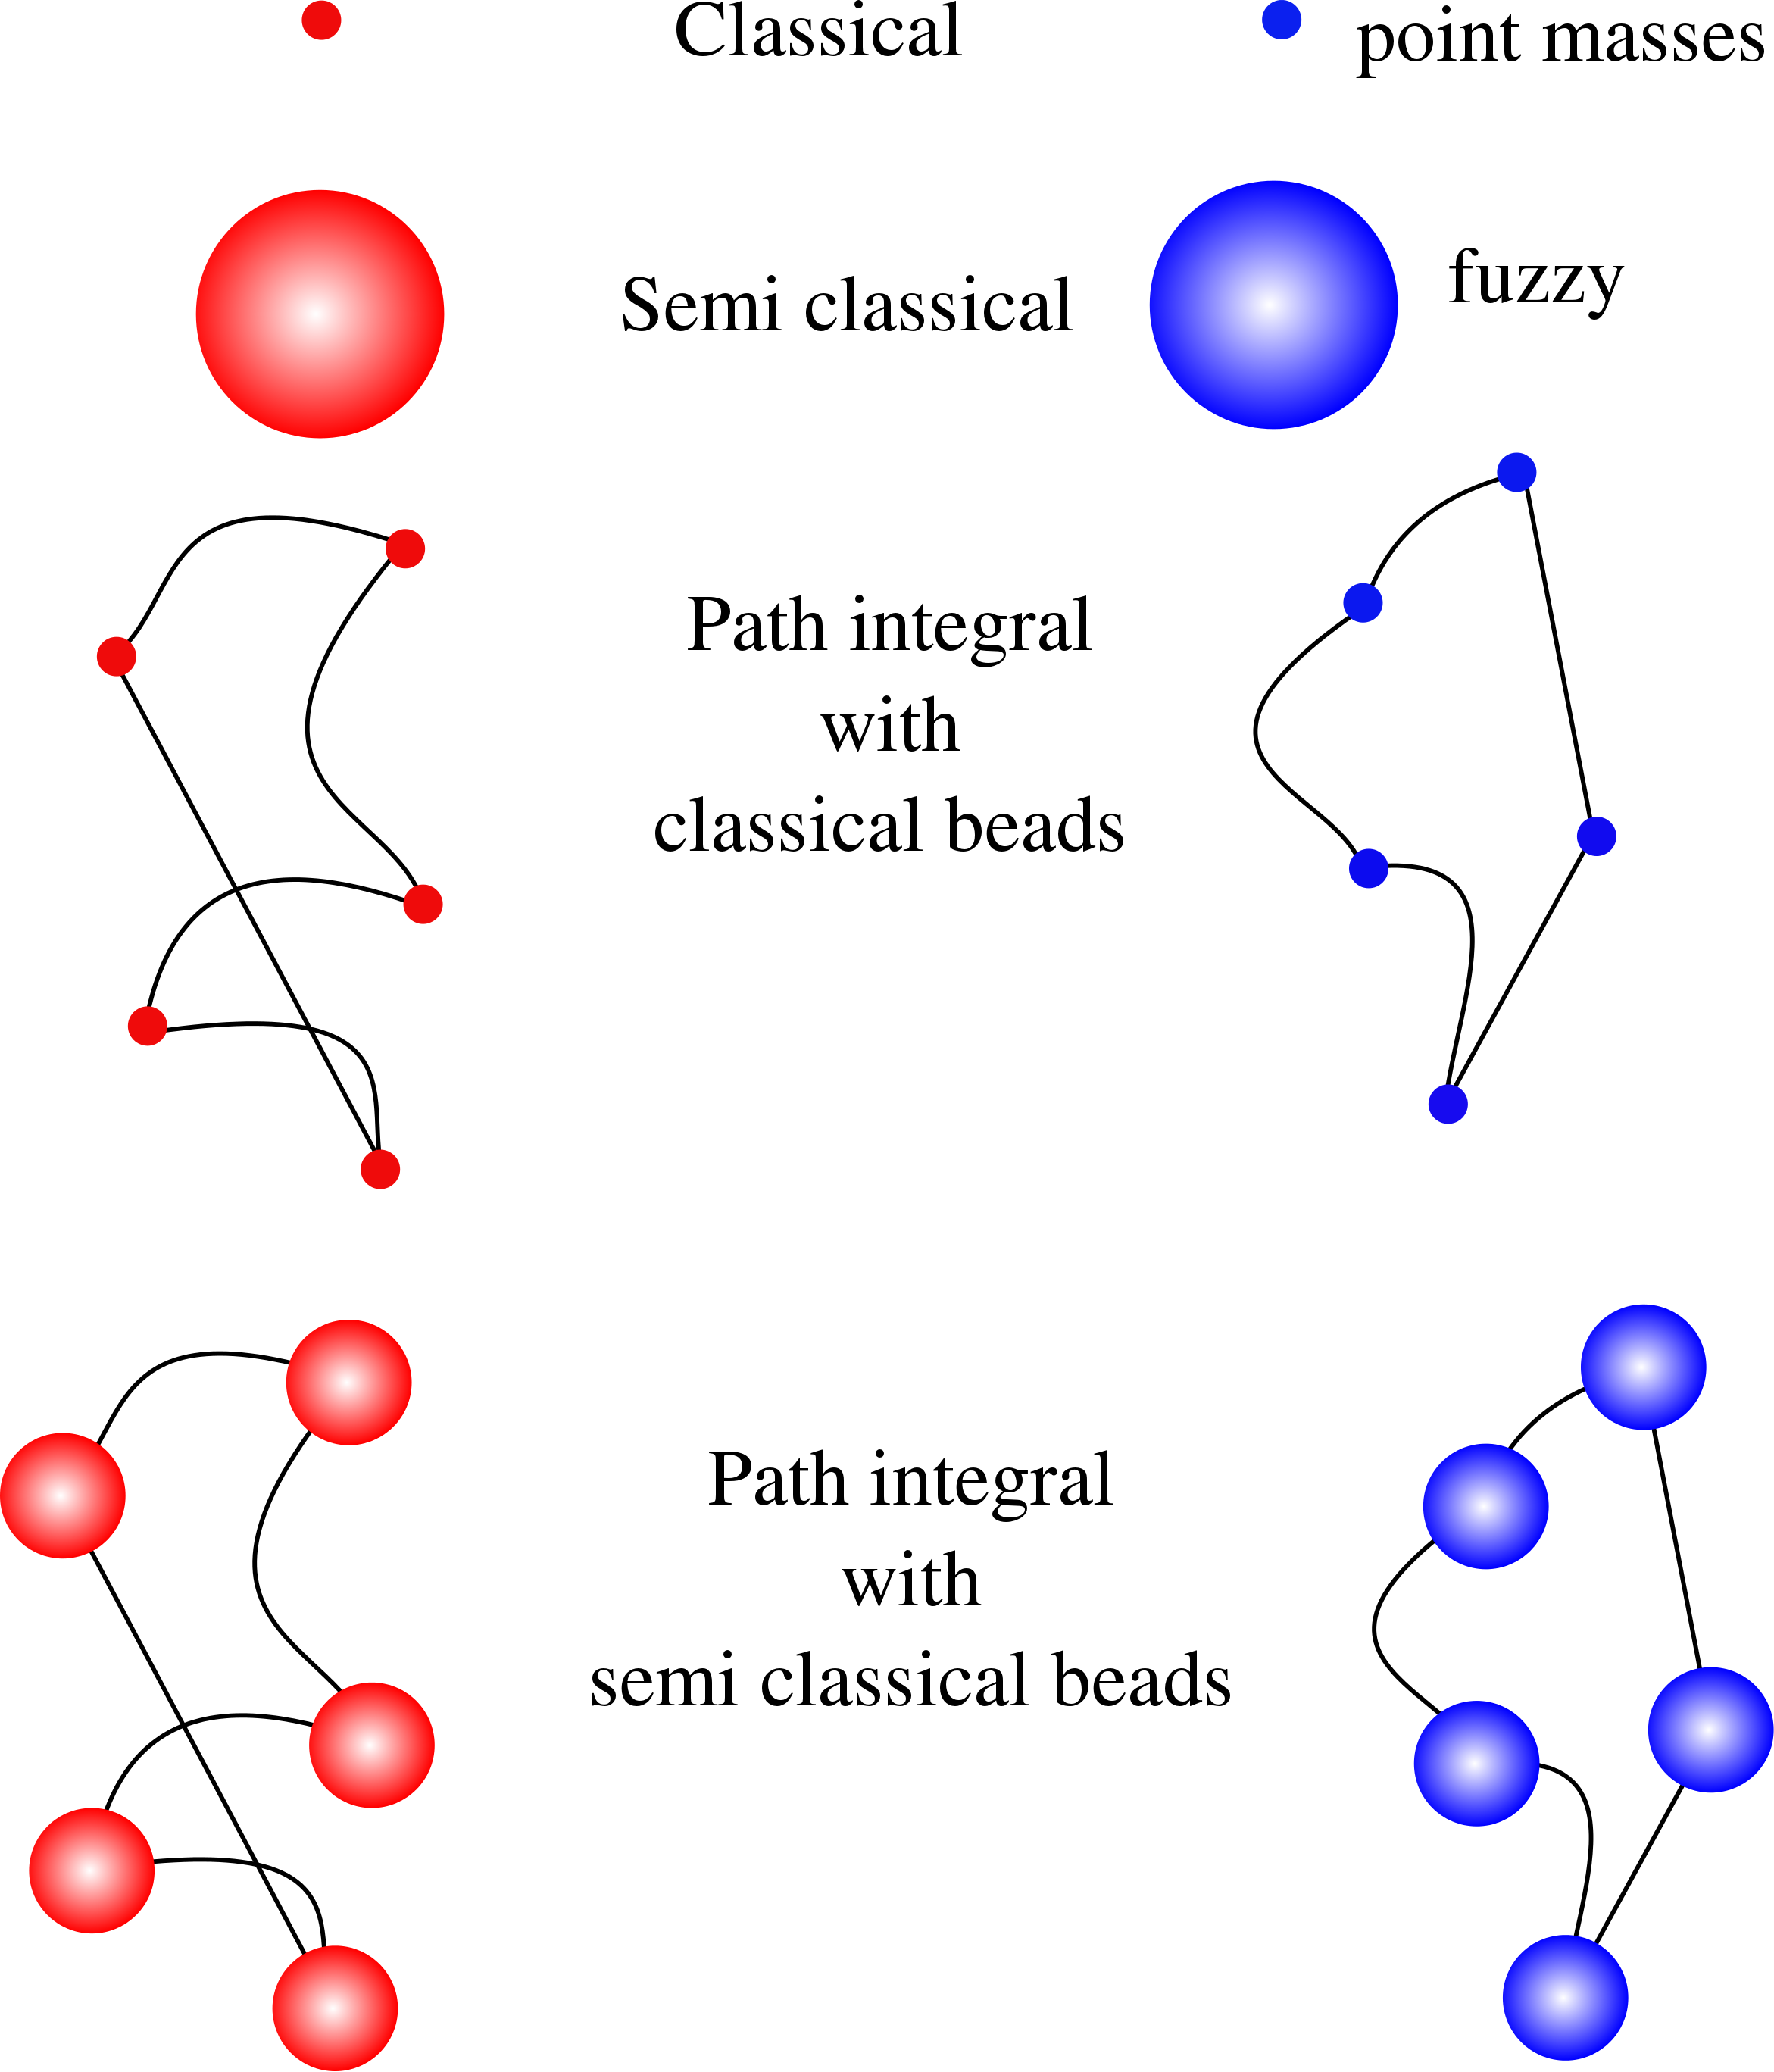
\includegraphics[scale=0.087,keepaspectratio]{Chapter-2/Figures/quantumLevels.png}
                \caption{Different levels of ``quantumness" of a $B_2$ calculation going from classical virial coefficients that are calculated assuming point masses to fully quantum virial coefficients with semi-classical beads. The different sphere sizes here are for illustrative purposes only and no quantitative inference should be made.} \label{quantumness}
            \end{figure}
\section{Existing algorithms}
\section{Novel algorithms}
